%!TeX root = ../My_thesis.tex


%% ---------- chapter ---------- %%
\chapter{Особенности обработки японского языка}\label{ch1}
%% ---------- chapter ---------- %%


%% ---------- section ---------- %%
% \section{Особенности обработки японского языка}
%% ---------- section ---------- %%


%% ---------- subsection ---------- %%
\section{Японская письменность}
%% ---------- subsection ---------- %%


Японский является очень неординарным языком, сильно отличающимся от европейских, в том числе от русского и английского.
На это очень сильно повлиял тот факт, что Япония на протяжении многих веков была закрытой страной для большей части мира.
Тем не менее, довольно значимое влияние на японский оказал китайский язык, из которого японцы взяли иероглифы, которые в Японии называют кандзи, но в отличие от китайцев, японцы используют также 2 слоговые азбуки "--- хирагану и катакану.
Примеры японской письменности показаны на~\firef{japanese-writing}.

\begin{figure}[H]%
  \centering
  \begin{tabular}{ll}
    Катакана: & \jp{オマエハモウシンデイル} \\ 
    Хирагана: & \jp{おまえはもうしんでいる} \\ 
    Кандзи: & \jp{夜露死苦}
  \end{tabular}
  \caption{Японская письменность}
  \label{japanese-writing}
\end{figure}


%% ---------- subsection ---------- %%
\section{Упрощение лексики}
%% ---------- subsection ---------- %%


Вместе с письменностью в японский язык пришло и немалое количество слов из китайского языка, вообще говоря, практически каждый иероглиф в японском имеет как минимум 2 чтения: онъёми (китайское чтение, хотя часто сильно отличающееся от изначального китайского звучания ввиду особенностей японской фонетики) и кунъёми (японское чтение).
Как правило (хоть и не всегда), лексика, пришедшая из китайского языка, значительно труднее исконно японских слов и зачастую упрощение текстов на японском состоит именно в замене таких слов на японские аналоги.
На~\firef{muzuiNaKore} показан пример упрощения редко встречающегося слова китайского происхождения вполне обычным повседневным лексиконом, состоящим из чисто японских слов и понятному любому школьнику.
Как можно заметить, упрощённый результат получился ощутимо длиннее изначального слова.

\begin{figure}[H]%
  \centering
  \begin{tabular}{rl}
    \yubi{\jp{知識豊富}}{chishiki houfu} & "--- редкое слово (знаток) \\ 
    \yubi{\jp{いろいろ}}{iroiro}%
    \yubi{\jp{な}}{na}%
    \yubi{\jp{こと}}{koto}%
    \yubi{\jp{を}}{wo}%
    \yubi{\jp{知っている}}{shitteiru} & "--- простой лексикон (много знающий) \\
  \end{tabular}
  \caption{Пример упрощения сложного слова}
  \label{muzuiNaKore}
\end{figure}


%% ---------- subsection ---------- %%
\section{Японская грамматика}
%% ---------- subsection ---------- %%


В японском, как и в китайском, не используются пробелы, что является существенной проблемой в задаче токенизации (разбиение текста на список токенов "--- отдельных слов, чисел, дат и~т.\,д.)
Существуют готовые решения в области токенизации для обоих языков, однако они сталкиваются с проблемами неоднозначности, которые нельзя решить без глубокого понимания текста и контекста.
Пример для японского, где 2 предложения абсолютно идентичны по написанию, но отличаются по смыслу, показан на~\firef{japanese-kek}.
Определить, что имеется в виду, можно лишь зная контекст этого предложения. 

\begin{figure}[H]%
  \centering
  \begin{tabular}{rl}
      \yubi{\jp{何で}}{\textbf{nande}}\yubi{\jp{来た}}{kita}\yubi{\jp{の}}{no}\jp{?}
    & "--- \textbf{зачем} ты приехал?
    \\ 
      \yubi{\jp{何}}{\textbf{nani}}\yubi{\jp{で}}{\textbf{de}}\yubi{\jp{来た}}{kita}\yubi{\jp{の}}{no}\jp{?}
      & "--- \textbf{на чём} ты приехал?
  \end{tabular}
  \caption{Пример неоднозначности в японском языке}
  \label{japanese-kek}
\end{figure}

Морфология в японском языке относительно простая "--- у слов нет ни числа, ни рода, ни падежей, отсутствуют артикли, у глаголов есть всего 2 времени: прошлое и настоящее-будущее.
Однако ввиду наличия очень большого количества омонимов (слов, звучащих или пишущихся одинаково, но имеющих разное значение, например, в словаре можно найти более 30 слов с написанием «shi»), могут возникать неоднозначности в письменности.
Как правило, в письменности омонимы различаются по иероглифам, используемым в словах, однако в текстах можно встретить эти слова, записанные азбукой, что и создаёт неоднозначности.
Такое большое количество омонимов появилось в японском из-за заимствования слов из китайского, где эти омонимы различались по тонам, которые в японском не используются.


% %% ---------- subsection ---------- %%
% \subsection{Раскрытие анафор в японском}
% %% ---------- subsection ---------- %%


% Несмотря на большое количество местоимений в японском языке (например, вариаций одного лишь местоимения «я» больше десяти), они используются довольно нечасто, особенно это касается слов «он» и «она», которые встречаются в основном лишь в переводах с других языков, где местоимения используются очень часто (например, в английском).
% Поэтому в японском не так остро обстоит проблема с раскрытием анафор (пониманием, что имеется в виду при использовании местоимений).


%% ---------- section ---------- %%
% \section{Существующие решения и датасеты}
%% ---------- section ---------- %%


%% ---------- chapter ---------- %%
\chapter{Существующие решения и датасеты}\label{ch2}
%% ---------- chapter ---------- %%


% %% ---------- subsection ---------- %%
% \subsection{Упрощённый корпус с базовым словарём}
% %% ---------- subsection ---------- %%


% Маруяма~Т. и Ямамото~К.


%% ---------- subsection ---------- %%
\subsection{Модель Transformer}
%% ---------- subsection ---------- %%


Маруяма~Т. и Ямамото~К. использовали в своём исследовании~\cite{Transformer2019} относительно новую модель Transformer~\cite{vaswani2017attention}.
Они предобучили свою модель на статьях с японской википедии, после чего дообучили (fine-tune) её на небольшом параллельном корпусе, состоящим из 1\,100 документов, составленных 40 учителями японского языка~\cite{moku-yamamoto-2012-automatic}.
Авторы показали, что в условиях малого количества ресурсов (отсутствия объёмных корпусов для упрощения японских текстов), модель Transformer показывает довольно хорошие результаты "--- она существенно обходит существующие на сегодняшний день решения в обоих метриках BLEU и SARI, которые обычно используют в задаче упрощения текстов.


%% ---------- subsection ---------- %%
\subsection{Улучшение упрощения увеличением корпуса с обучением без учителя}
%% ---------- subsection ---------- %%


Кацута~А. и Ямамото~К. попробовали создать модель, не требующую параллельного корпуса, то есть их модель может обучаться без учителя~\cite{Unsupervised2019}.
Их подход заключается в создании псевдокорпуса из неразмеченного веб-корпуса, они показали, что расширение такого корпуса ведёт улучшению результатов упрощения.


%% ---------- subsection ---------- %%
\subsection{JSSS корпус}
%% ---------- subsection ---------- %%


Такамичи~С., Комачи~М. и~др. составили корпус для упрощения и реферирования японской речи~\cite{takamichi2020jsss}.
Корпус содержит проговорённые дикторами тексты, для каждого текста есть таймкоды для синхронизации текста и речи, для упрощения есть параллельные упрощённые тексты, для реферирования, соответственно, приведены рефераты текстов.
Тем не менее размер данного корпуса довольно мал "--- он содержит лишь несколько сотен предложений, "--- поэтому за основу его брать нельзя, однако его можно попробовать использовать для объединения с другими корпусами. 


%% ---------- section ---------- %%
% \section{Где используют упрощение}
%% ---------- section ---------- %%


%% ---------- chapter ---------- %%
\chapter{Где используют упрощение}\label{ch3}
%% ---------- chapter ---------- %%


Для английского языка существует упрощённая википедия, где статьи вручную переведены в упрощённый вариант английского (Simple English), использующий приблизительно 1\,500 одних из наиболее употребляемых английских слов.
Simple English основан на Basic English, использующий 850 слов, созданный Чарльзом К. Огденом.
На ноябрь 2020 упрощённая википедия содержит более 177\,000 статей~\cite{SimpleWiki}.

Чего-то столь же масштабного для японского языка не существует.
Есть новостной сайт News Web Easy, на котором выкладывают упрощённые версии новостей NHK (одна из крупнейших японских СМИ) для учеников младшей и средней школ (дети до 15 лет) и иностранцев, проживающих в Японии.
Главная страница сайта показана на~\firef{NHK}.
Как и на Simple Wikipedia, упрощение новостей на News Web Easy происходит вручную~\cite{NHKnews}.
\begin{figure}[H]%
  \centering
  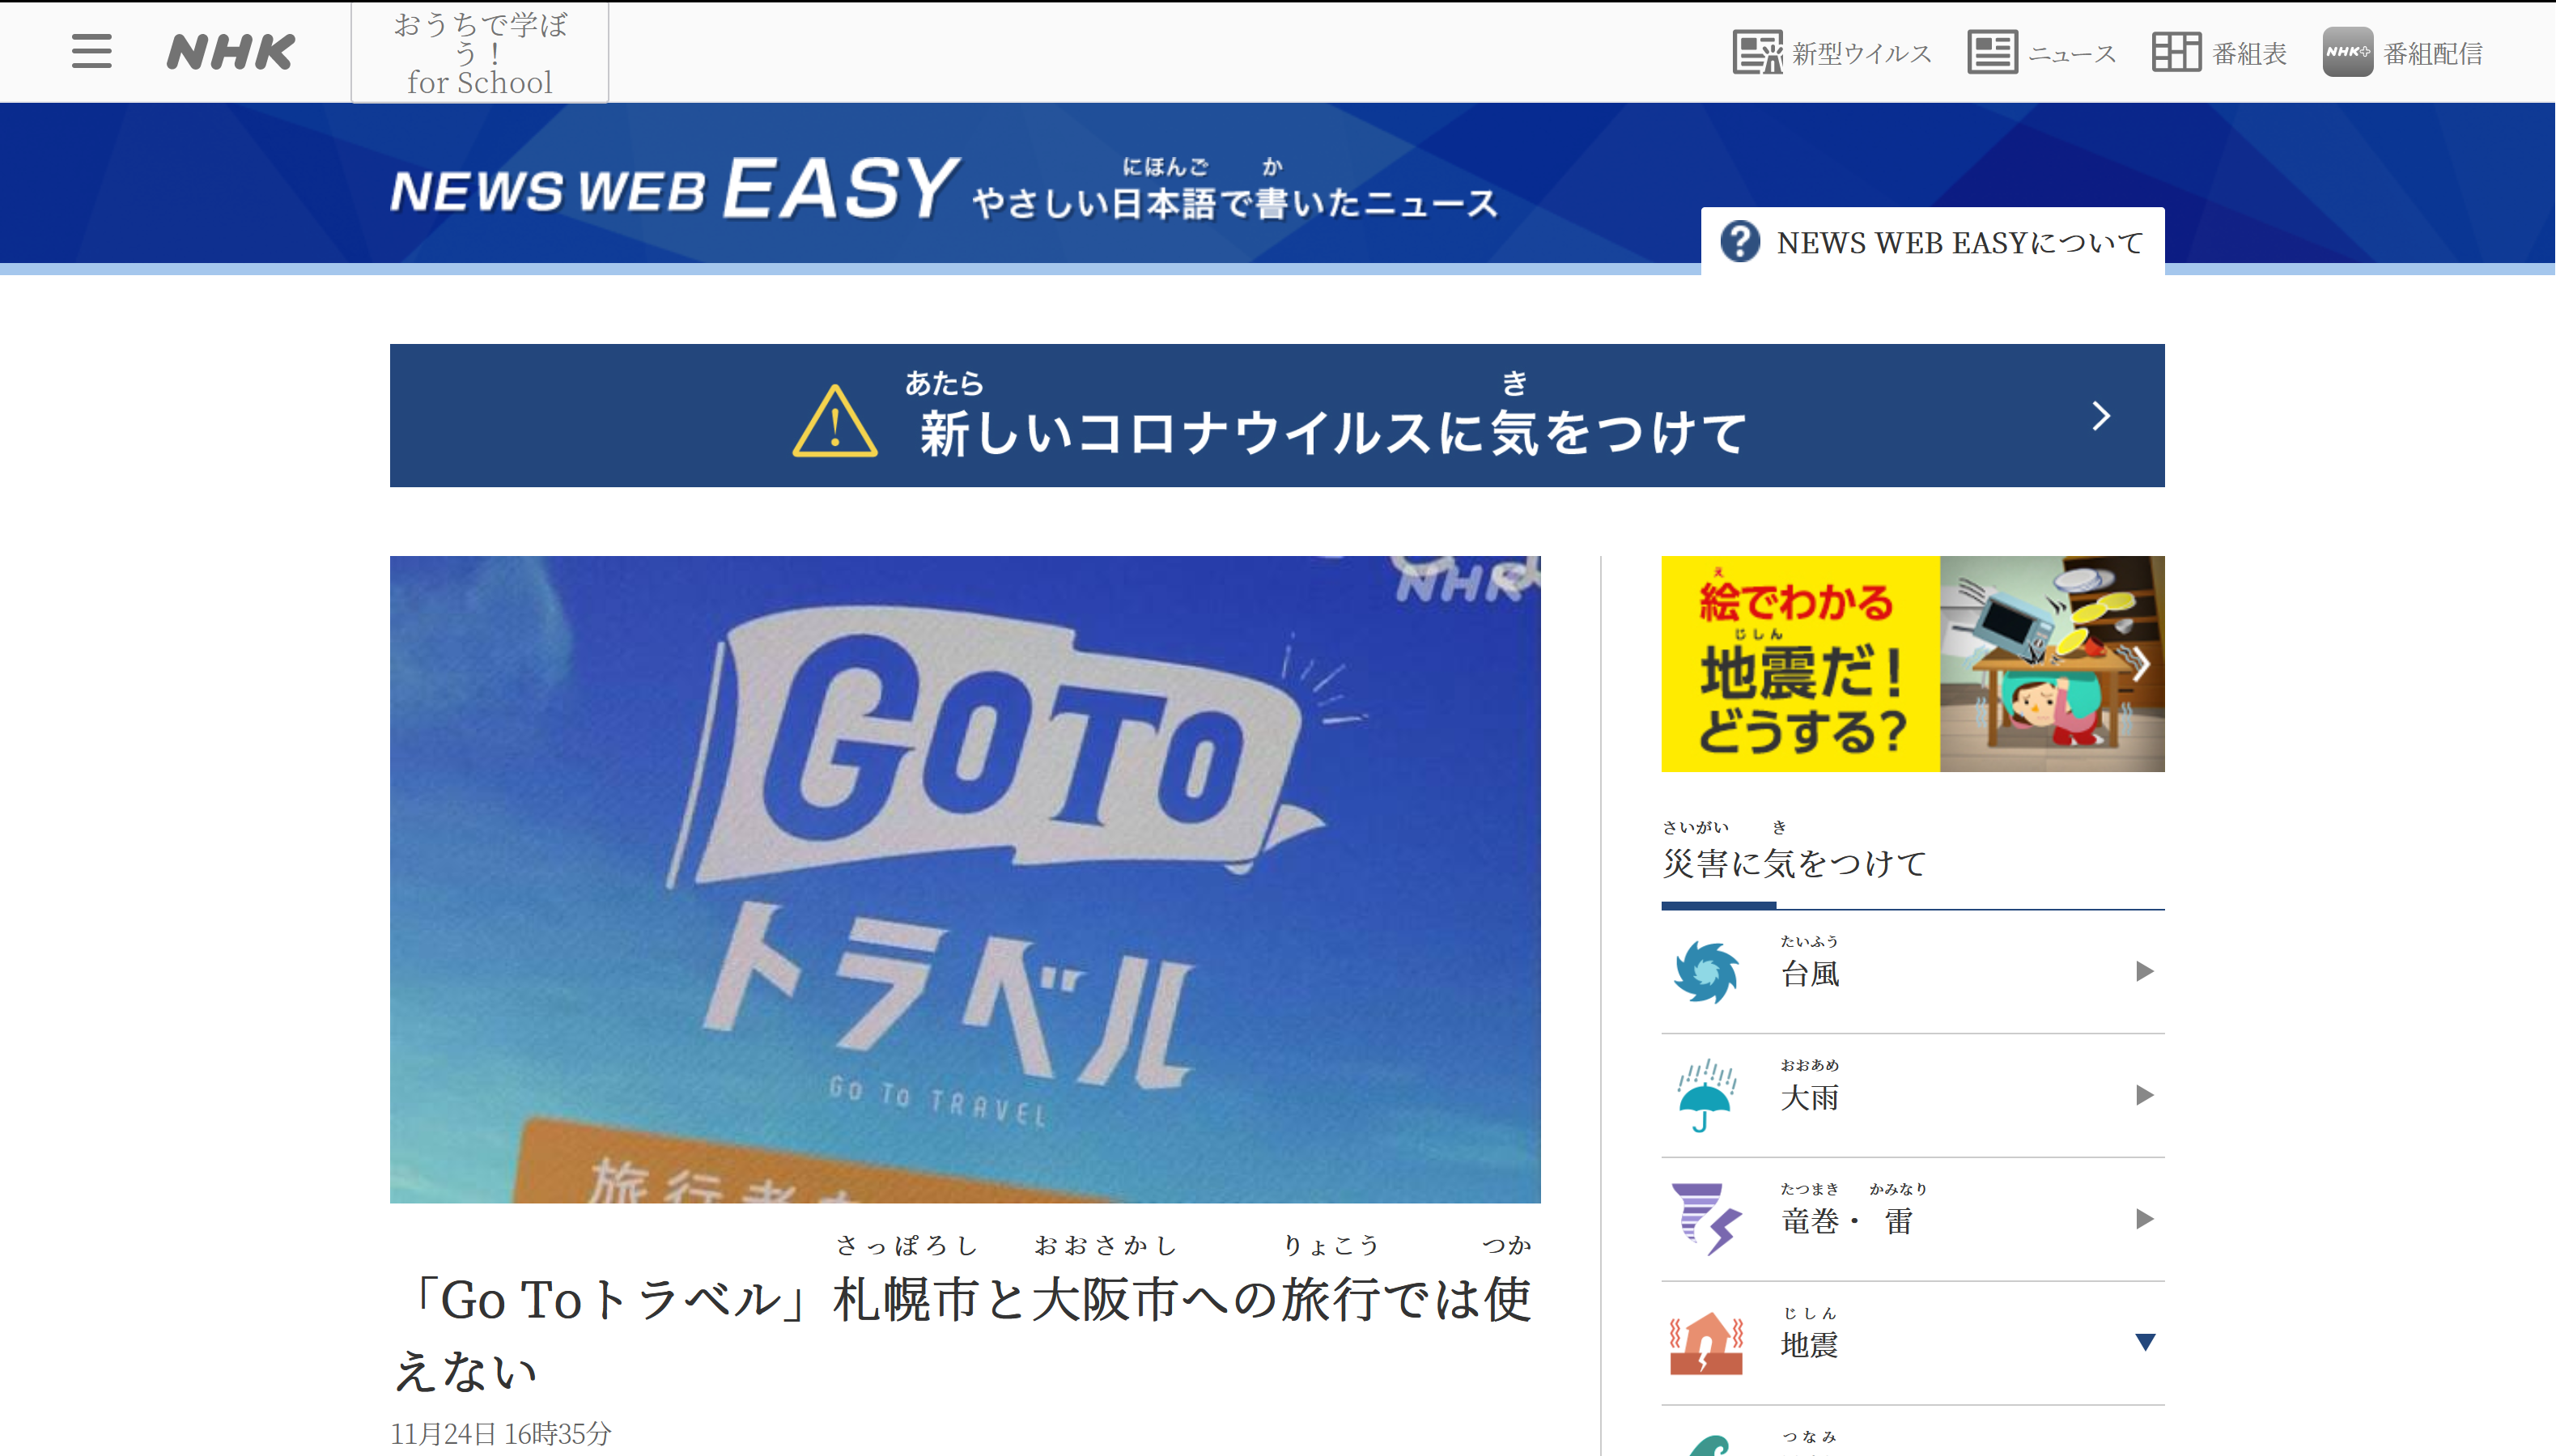
\includegraphics[width=\textwidth]{NHKniYoukoso.png}
  \caption{Главная страница News Web Easy}
  \label{NHK}
\end{figure}

Вообще говоря, на сегодняшний пока ещё день не существует достаточно качественной системы упрощения текстов, способной заменить ручной перевод "--- дела здесь обстоят немногим лучше машинного перевода (из одного языка в другой), что можно объяснить отсутствием качественного и масштабного корпуса для обучения модели упрощения текстов (не только для японского языка, но даже для английского) и довольно высокой сложностью самой задачи, связанной с необходимостью «понимать» текст, что, к сожалению, современный искусственный интеллект сделать пока ещё не в состоянии.

Тем не менее, подобно тому, как сегодня используются системы машинного перевода (например, перевод отдельных слов или перевод текстов с последующими ручными корректировками), могут использоваться и системы упрощения текстов.
